\documentclass{article}

\usepackage{caption}
\usepackage{subcaption}

\usepackage[margin=1in]{geometry}
\usepackage{custom}

\usepackage{apacite}
\usepackage{natbib}
\usepackage{hyperref}


\title{Adaptive Optics Imaging of Neptune \\ ASTR 257: Observational Astronomy}
\author{Aditya Sengupta}

\begin{document}
    \maketitle
    \section{Observations}

    We analyzed adaptive optics observations of Neptune taken in three filters in order to make a three-color image. Due to poor weather conditions on the scheduled night, data from the 2019 iteration of this class, taken by Arcelia Hermosillo Ruiz, were used for reductions and results \footnote{data available at \href{https://github.com/askemer/ASTR257\_2019}{https://github.com/askemer/ASTR257\_2019}}. These data were taken with the ShARCS near-infrared camera on the Shane telescope at Lick Observatory\citep{sharcsmcgurk}. Conditions were photometric with a seeing of 1.25 arcseconds. Images were taken in three filters:

    \begin{enumerate}
        \item J, with a central wavelength of 1.238 $\mu$m;
        \item H, with a central wavelength of 1.656 $\mu$m;
        \item Ks, with a central wavelength of 2.150 $\mu$m.
    \end{enumerate}
    
    Sky flats were taken starting at UT 2019-09-27 01:50:10 and science images were taken starting at UT 2019-09-27 03:14:11. The AO system creates a circular image on the detector with a diameter of 840 pixels out of the overall grid of 2048$\times$2048 pixels. The unvignetted square within this circle covers a field of view of 20 $\times$ 20 arcseconds, so the circle's diameter is $20\sqrt{2} \approx 28.28$ arcseconds\footnote{This information is from the ShARCS documentation at \href{https://mthamilton.ucolick.org/techdocs/instruments/sharcs/intro/}{https://mthamilton.ucolick.org/techdocs/instruments/sharcs/intro}}. This gives us a plate scale of $\frac{28.28}{840} \approx 0.033$ arcsec/px. 1x binning was chosen, likely in order to maximize the resolution of the final image.
    
    \begin{table}
        \centering
        \begin{tabular}{|c|c|c|c|}
            \hline
            \textbf{Type of frame} & \textbf{Filter} & \textbf{Exposure time} & \textbf{Number}\\
            \hline
            Flat field & H & 7.5 s & 15\\
            Flat field & J & 6 s & 15\\
            Flat field & Ks & 30 s &  11\\
            Science & H & 120 s & 5\\
            Science & J & 120 s & 4\\
            Science & Ks & 120 s & 5\\\hline
        \end{tabular}
        \caption{The flat-field and science frames being analyzed}
        \label{tab:frames}
    \end{table}

    Science images were taken using a four-point dither with a separation of 7.5 arcseconds. The first image in H and in Ks was disregarded as the same position was used in one of the later frames.

    \section{Reductions}

    The raw frames were flat-fielded. Since the flat-field images were taken on sky at twilight, the earlier frames had higher levels of background illumination than the later ones. In order to compensate for this, we take the pixel-by-pixel median of the flats, and further normalize by dividing each by their overall median across the whole image. This removes a brightness gradient across the uncalibrated images. There were no bias frames or dark current frames, so we do not consider dark current. 

    The AO system produces images on a region contained within the CCD, so we crop each science image to a 500 $\times$ 500 cutout within this region. In order to make Neptune more apparent so that offset calculations identify the correct point, we rescale the cropped images using ds9's \textit{zscale} parameters as a reference, so that the brightest pixel is no brighter than the zscale maximum and the faintest is no fainter than the \textit{zscale} minimum. This improved the performance of the subsequent offset calculation.

    We took the median science image within each filter and subtracted it from each individual science image. Taking the pixel-by-pixel median removes Neptune, as there are more images being medianed that do not have Neptune in a particular position than those that do, so the median value can be subtracted from each image without introducing negative copies of the target. 

    \begin{figure}
        \centering
        \begin{subfigure}[b]{0.3\textwidth}
            \centering
            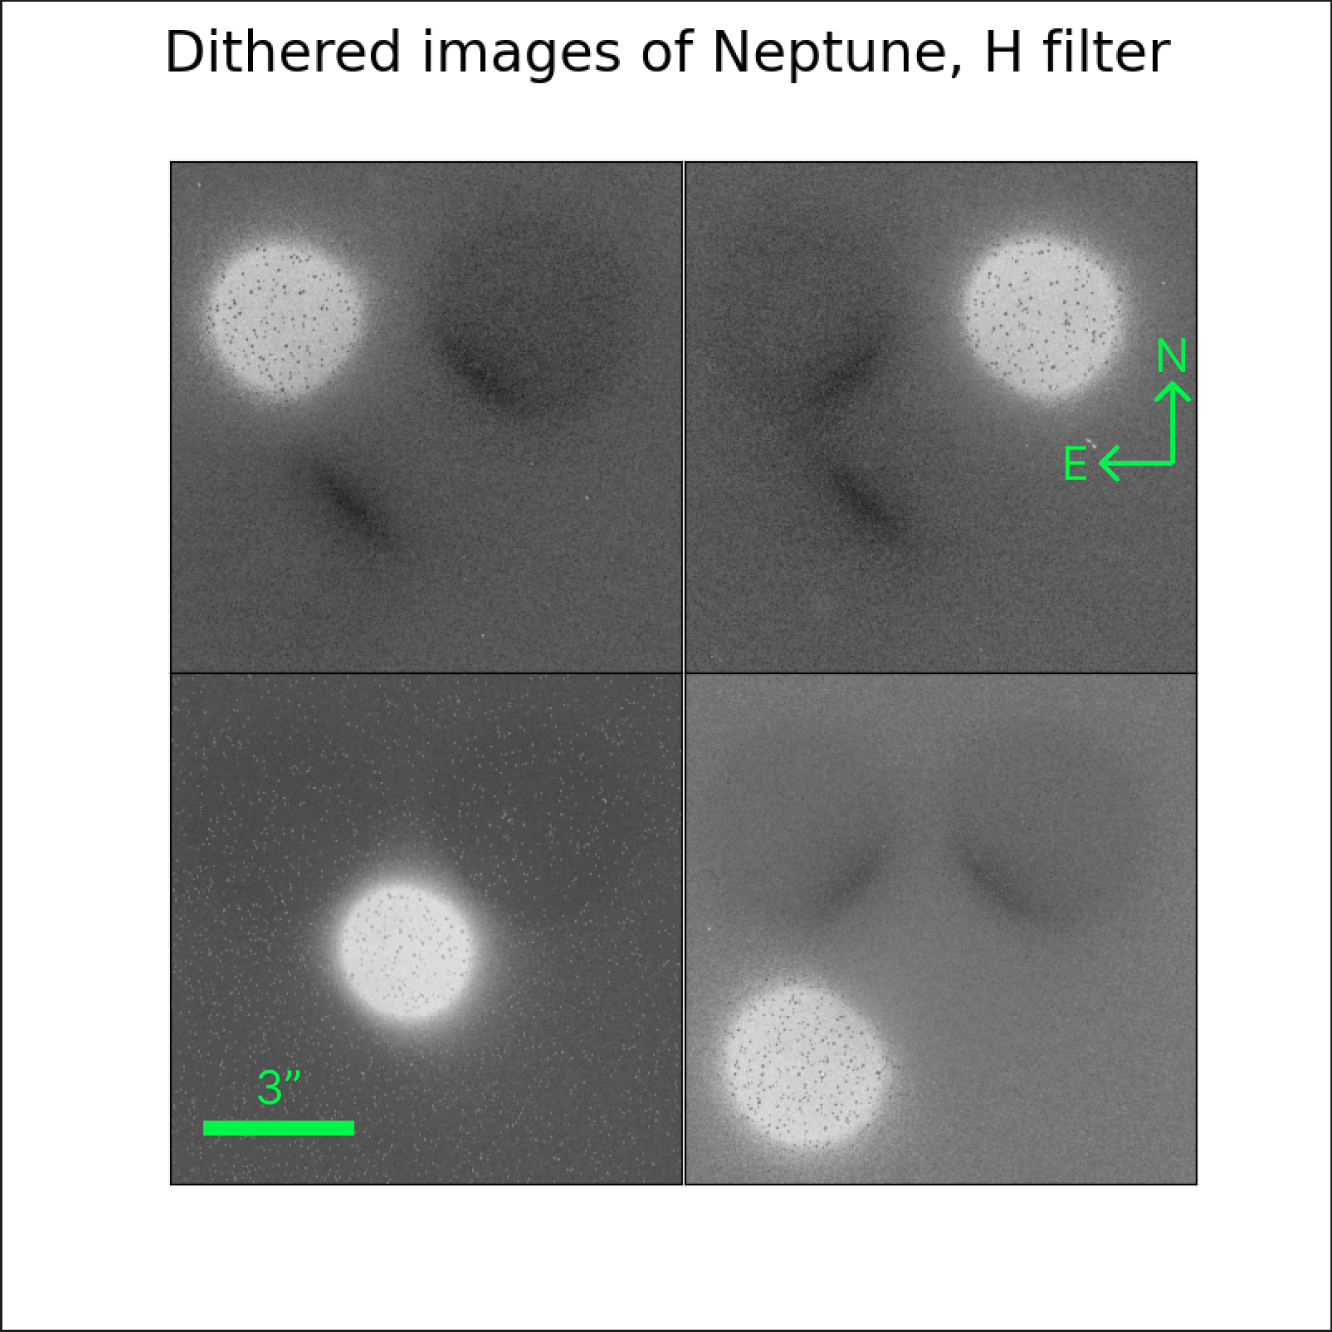
\includegraphics[width=\textwidth]{uncorr_H_sc.png}
            \caption[uncorr H]%
            {{\small H filter}}    
            \label{fig:uncorr_H}
        \end{subfigure}
        \hfill
        \begin{subfigure}[b]{0.3\textwidth}
            \centering
            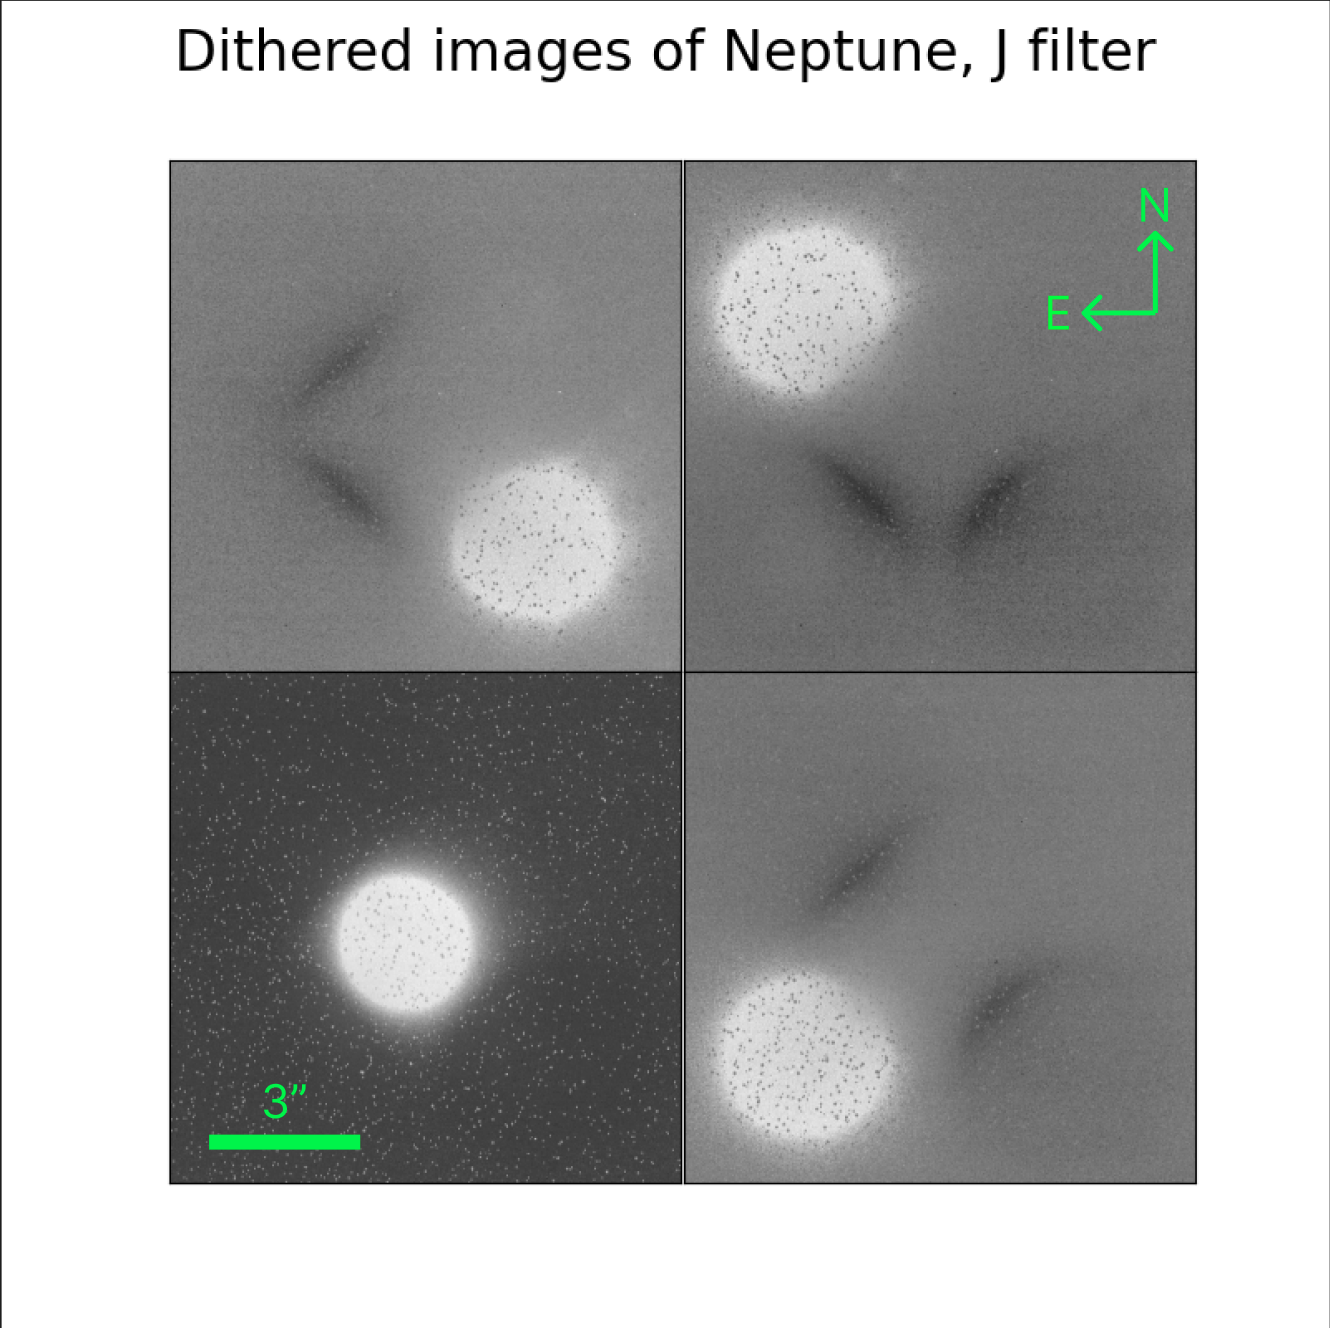
\includegraphics[width=\textwidth]{uncorr_J_sc.png}
            \caption[uncorr J]%
            {{\small J filter}}    
            \label{fig:uncorr_J}
        \end{subfigure}
        \hfill
        \begin{subfigure}[b]{0.3\textwidth}
            \centering
            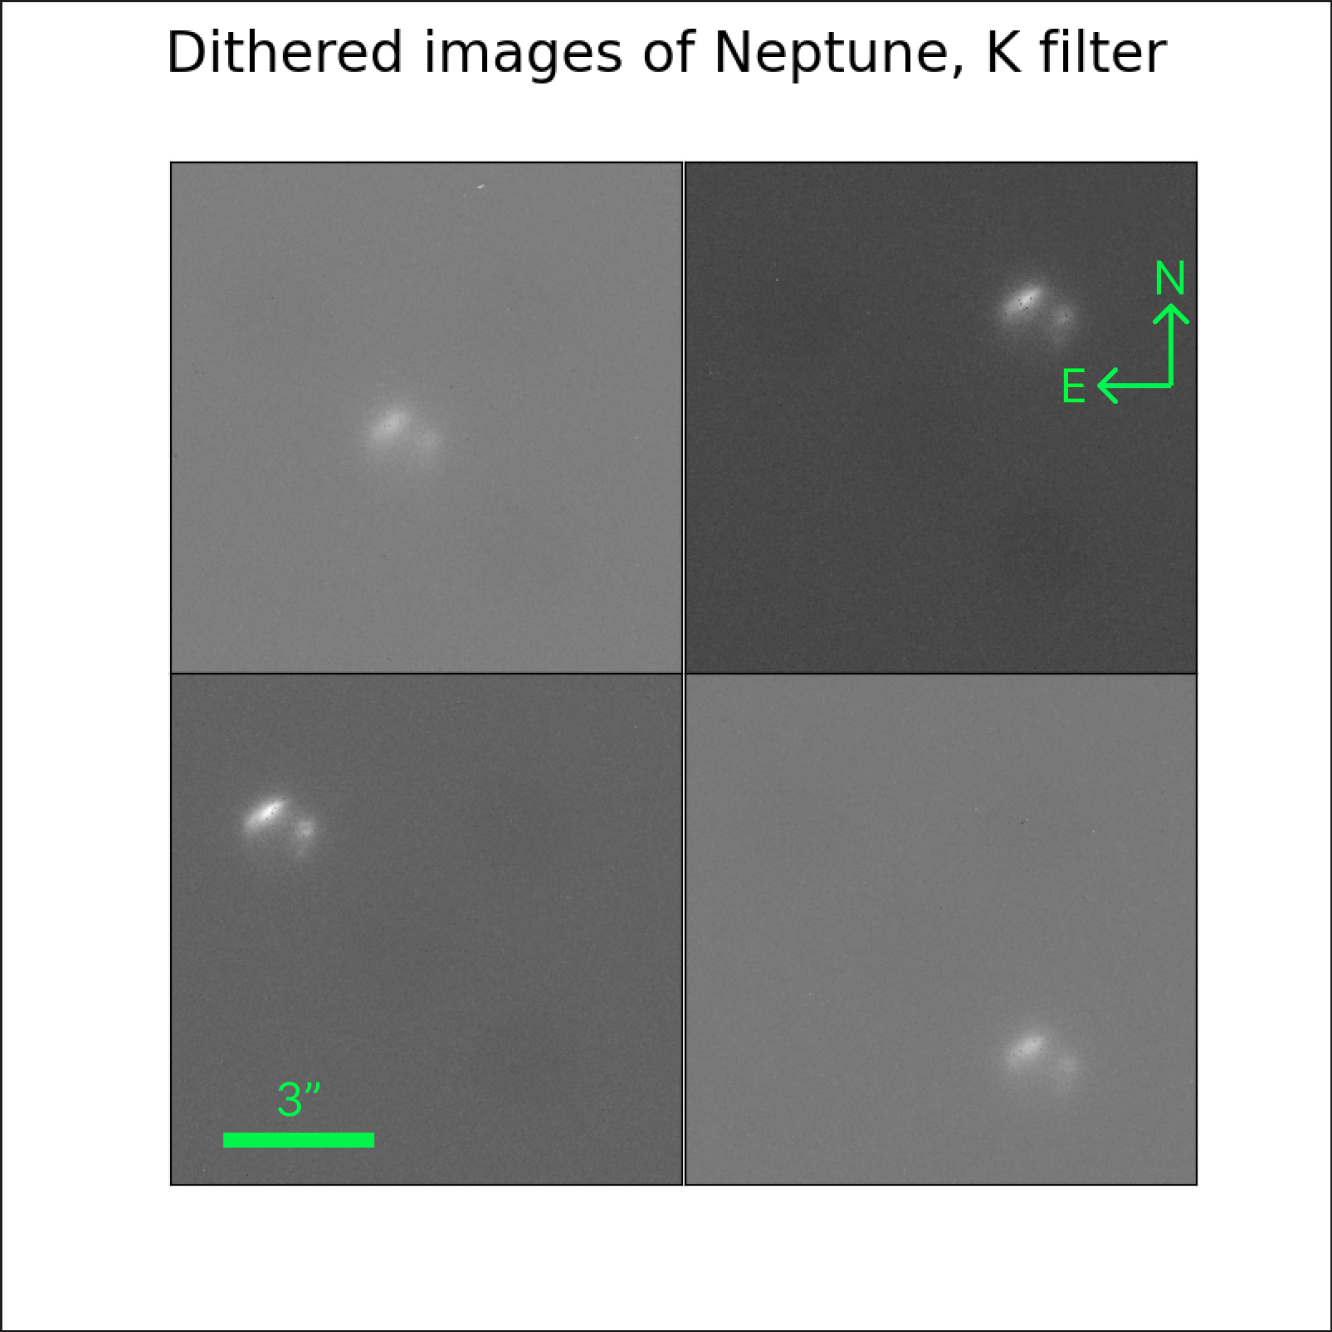
\includegraphics[width=\textwidth]{uncorr_K_sc.png}
            \caption[uncorr Ks]%
            {{\small Ks filter}}    
            \label{fig:uncorr_Ks}
        \end{subfigure}
        \caption{The science images prior to offset correction.}
        \label{fig:uncorr_images}
    \end{figure}

    We computed the offset of each image relative to the first frame in the H filter using the \textit{chi2\_shift} method from the \textit{image\_registration} Python package\citep{imagereg}, and applied these offsets using the \textit{shift.shiftnd} method from the same package. Figure~\ref{fig:uncorr_images} shows each dithered image prior to applying offsets, and Figure~\ref{fig:corr_images} shows the same images after the shifts had been applied.

    \begin{figure}
        \centering
        \begin{subfigure}[b]{0.3\textwidth}
            \centering
            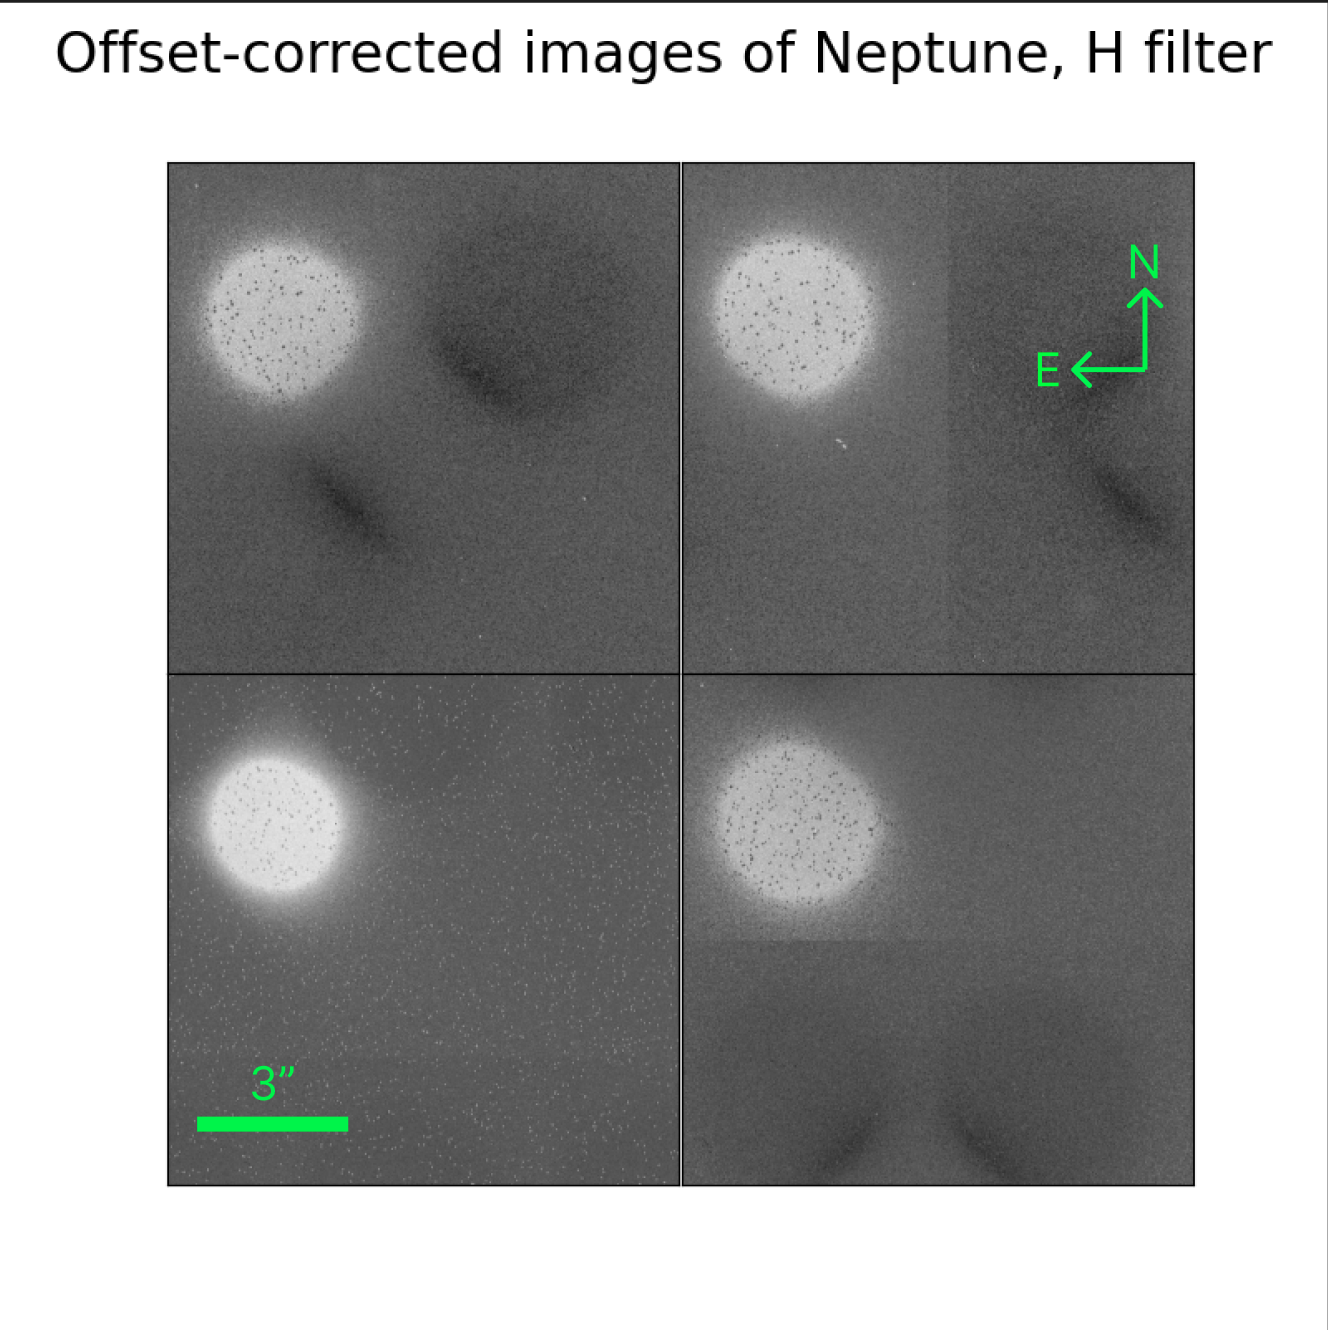
\includegraphics[width=\textwidth]{corr_H_sc.png}
            \caption[corr H]%
            {{\small H filter}}    
            \label{fig:corr_H}
        \end{subfigure}
        \hfill
        \begin{subfigure}[b]{0.3\textwidth}
            \centering
            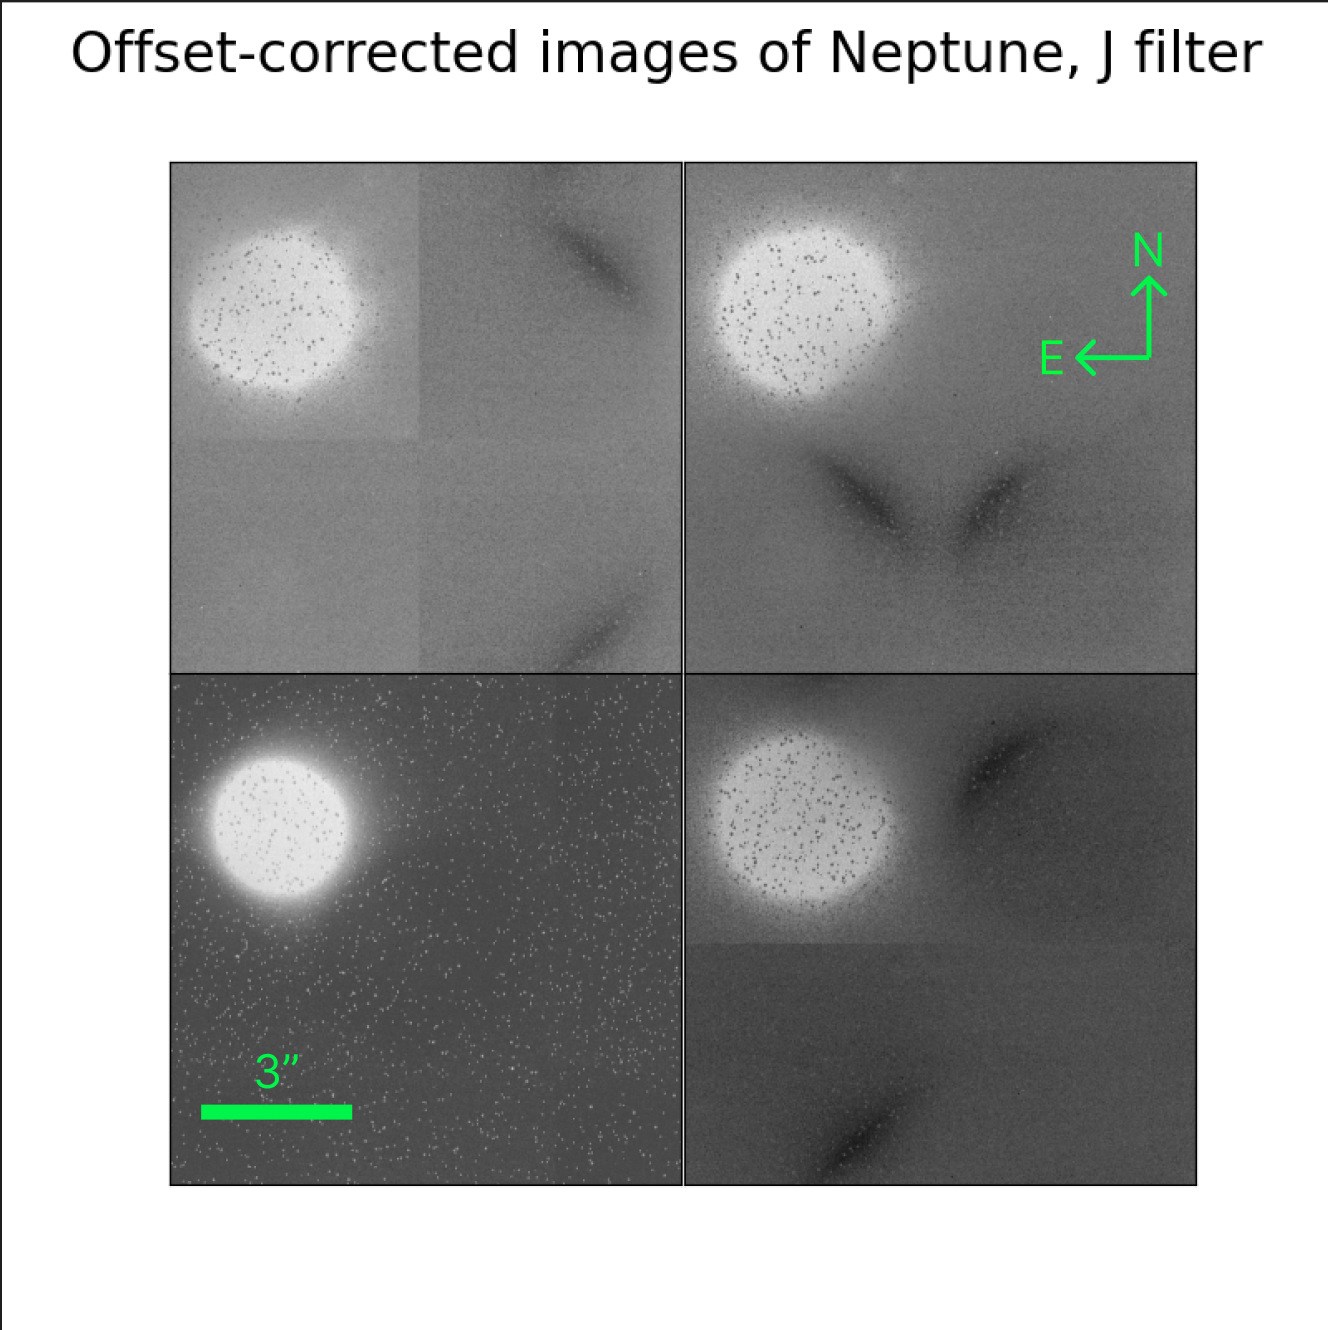
\includegraphics[width=\textwidth]{corr_J_sc.png}
            \caption[uncorr J]%
            {{\small J filter}}    
            \label{fig:corr_J}
        \end{subfigure}
        \hfill
        \begin{subfigure}[b]{0.3\textwidth}
            \centering
            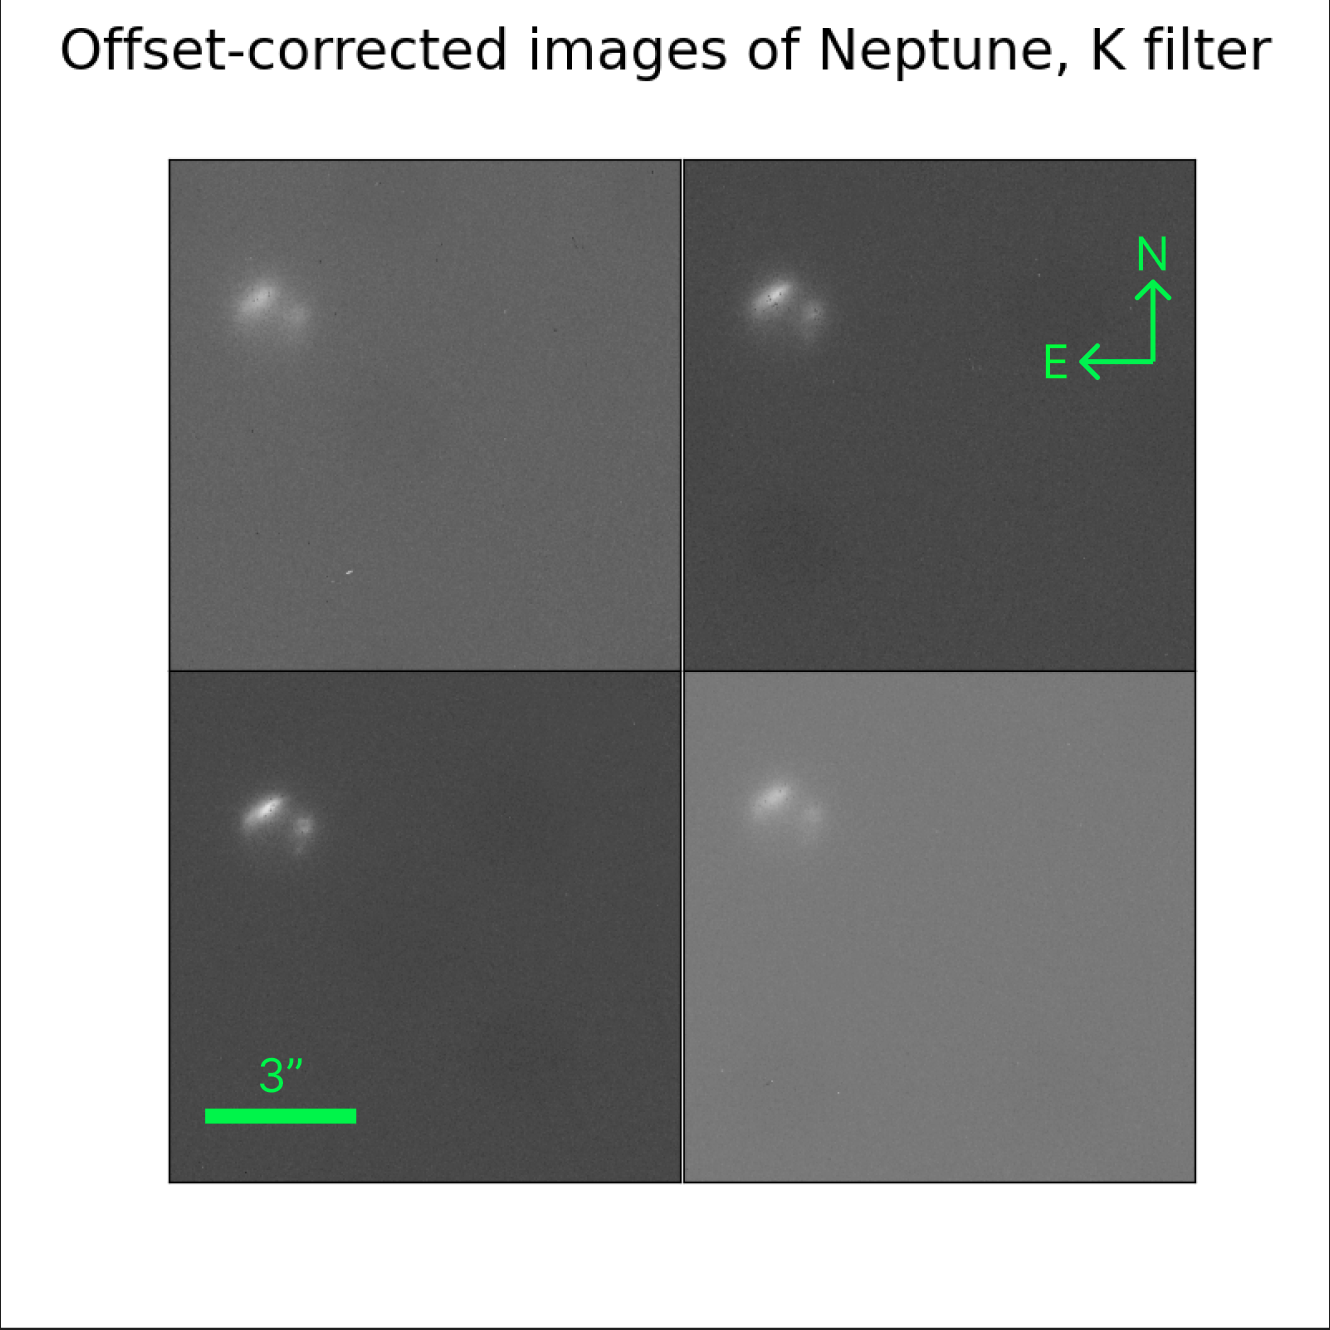
\includegraphics[width=\textwidth]{corr_K_sc.png}
            \caption[uncorr Ks]%
            {{\small Ks filter}}    
            \label{fig:corr_Ks}
        \end{subfigure}
        \caption{The offset-corrected science images.}
        \label{fig:corr_images}
    \end{figure}

    We took the mean of the four resulting images in each filter to get the final image per channel. In order to make the three-color image, we use the Ks image in the red channel, the H image in the green channel, and the J image in the blue channel, to match the order of the colors to the order of the central wavelength of each filter.

    Figure~\ref{fig:threecolor} shows the final image.

    \begin{figure}
        \centering
        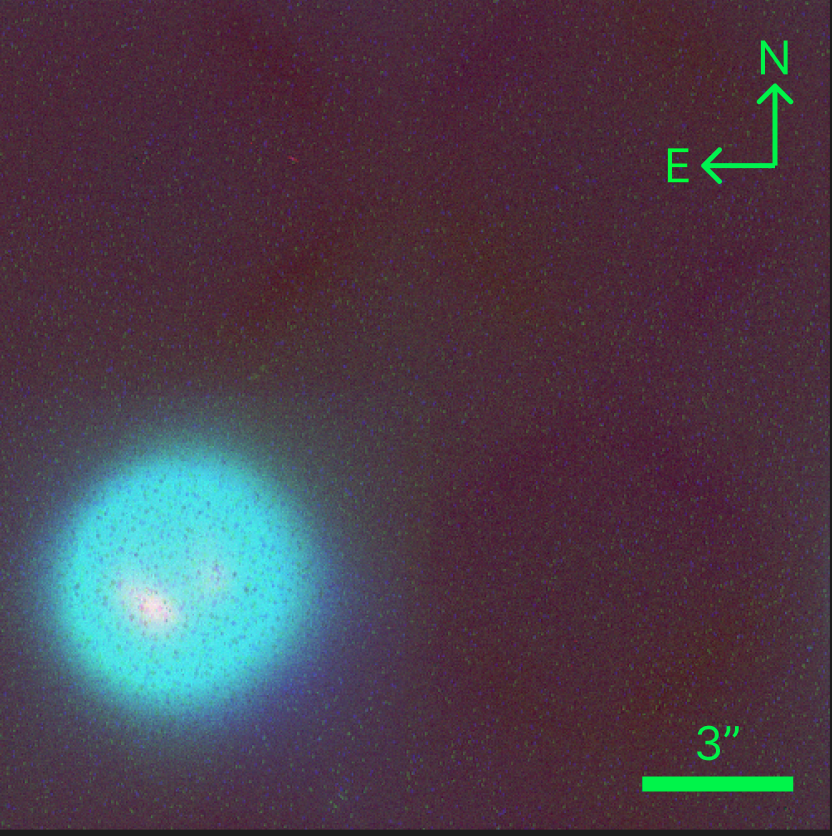
\includegraphics[width=\textwidth]{neptune_final_sc.png}
        \caption{The final three-color image.}
        \label{fig:threecolor}
    \end{figure}

    \bibliography{ao}{}
    \bibliographystyle{apacite}
\end{document}